\documentclass[main.tex]{subfiles}
\begin{document}
\chapter{Wahrscheinlichkeitstheorie}
\chapterauthor{Rémy}

\begin{Bemerkung}
  Der Oberbegriff \textbf{Stochastik} wird hier nicht verwendet, da wir uns SMP nicht mit der überflüssigen \textbf{Statistik} beschäftigen.
\end{Bemerkung}
\section{Wiederholungen: Unter- \& Mittelstufe}
\subsection{Zufallsexperimente}
\begin{Definition}
  Als Zufallsexperiment bezeichnet man Versuche, deren Ergebnisse sich nicht vorhersagen lassen, also vom Zufall abhängig sind.\\
  Vor der Durchführung eines Zufallsexperiments muss eine \textbf{Ergebnismenge} $S$ festgelegt werden. Sie beinhaltet alle möglichen Ergebnisse: $S = \{ e_1, e_2, ..., e_n \} $\\
  Ein Versuch heißt Zufallsexperiment, falls:
  \begin{itemize}
    \item er unter gleichen Bedingungen beliebig oft wiederholbar ist
    \item alle möglichen Ergebnisse vor Durchführung bekannt sind
    \item sein Ergebnis sich nicht mit Sicherheit vorhersagen lässt
    \item bei jeder Durchführung genau ein Ergebnis aus $S$ auftritt
  \end{itemize}
\end{Definition}
\begin{Beispiel}
  Bekannte Zufallsexperimente sind:
  \begin{itemize}
    \item das Werfen einer Münze
    \item das Werfen eines Würfels
    \item das Ziehen einer Kugel aus einer Urne
    \item ...
  \end{itemize}
\end{Beispiel}
\begin{Definition}[Laplace-Experiment]
  Laplace-Experimente sind Experimente, deren Ergebnisse jeweils gleichwahrscheinlich sind.
\end{Definition}
\begin{Beispiel}
  Ein Beispiel hierfür wäre der Wurf eines \textbf{perfekten} Würfels.
\end{Beispiel}
\begin{Theorem}
  In einem Laplace-Experiment gilt für die Wahrscheinlichkeit $P$, dass ein Ergebnis $A$ von $n$ möglichen Ergebnis eintritt:
  $$P(A)=\dfrac{1}{n}$$
\end{Theorem}
\subsubsection{Mehrstufige Zufallsexperimente}
\begin{Definition}
  Werden mehrere ($n$) Zufallsexperimente nacheinander ausgerführt, so kann man sie als ein einziges Zufallsexperiment zusammenfassen. Man nennt dies ein \textbf{mehrstufiges Zufallsexperiment}. Die Ergebnisse eines solchen Experiments kann man als geordnete $n$-Tupel auffassen.
\end{Definition}
\begin{Beispiel}
  Zweifaches Werfen einer Münze: $S=\{ (Z/Z),(Z/K),(K/Z),(K/K)\} $.\\
\end{Beispiel}
\begin{Bemerkung}
  Alternativ kann man $S$ als einfache Menge definieren. Bei zweifachem Münzwurf wäre eine mögliche Darstellung $S = \{ 0,1,2\}$ mit der Anzahl an Kopf-Würfen als Ergebnis möglich.
\end{Bemerkung}
\subsubsection{Ereignisse}
\begin{Definition}[Ereignisse]
  Jede Teilmenge $A$ von der Ergebnismenge $S$ nennt man ein Ereignis. Endet das Zufallsexperiment mit einem Ergebnis aus $A$, sagt man: $A$ ist eingetreten.
\end{Definition}
\begin{Beispiel}
  Werfen eines Würfels: $S = \{ 1,2,3,4,5,6 \}$\\\\
  \begin{minipage}{0.4\textwidth}
    $A$: Augenzahl ist gerade:\\
    $B$: Augenzahl ist ungerade:\\
    $C$: Augenzahl ist Primzahl:\\
    $D$: Augenzahl $<7$:\\
    $E$: Augenzahl $=6$:\\
    $F$: Augenzahl $>6$:\\
  \end{minipage}
  \begin{minipage}{0.6\textwidth}
    $A = \{ 2,4,6 \}$\\
    $B = \{ 1,3,5 \}$\\
    $C = \{ 2,3,5 \}$\\
    $D =S$\\
    $E = \{ 6 \}$\\
    $F = \{ \}$
  \end{minipage}
\end{Beispiel}
\begin{Bemerkung}
  \begin{Definition}
    \begin{itemize}
      \item Ein Ereignis, das nur aus einem Ergebnis besteht, heißt \textbf{Elementarereignis}.
      \item $B=\bar A$ (A quer) ist das \textbf{Gegenereignis} von $A$. Es gilt: $B = S \backslash A$
      \item Ein Ereignis, das immer eintritt, heißt \textbf{sicheres Ereignis}
      \item Ein Ereignis, das niemals eintritt, heißt \textbf{unmögliches Ereignis}
    \end{itemize}
  \end{Definition}
\end{Bemerkung}

\subsubsection{Baumdiagramme}
\begin{Definition}[Bernoulli-Experiment]
  Bei Bernoulli-Experimenten gibt es nur $2$ mögliche Ausgänge: Erfolg / Miserfolg ($= \overline{\text{Erfolg}}$). Mehrfaches Ausführen ($l$ Mal) von Bernoulli-Experimenten ergibt eine \textbf{Bernoulli-Kette} der Länge $l$.
\end{Definition}

Eine Bernoulli-Kette kann als \textbf{Baumdiagramm} dargestellt werden:

\tikzstyle{level 1}=[level distance=3.5cm, sibling distance=3.5cm]
\tikzstyle{level 2}=[level distance=3.5cm, sibling distance=2cm]
\tikzstyle{optionen} = [text width=4em, text centered]
\tikzstyle{ergebnis} = [circle, minimum width=3pt,fill, inner sep=0pt]
%Remove the sloped options to get horizontal labels.
\begin{center}
\begin{tikzpicture}[grow=right, ]%sloped]
\node[optionen] {\small{1. Durchführung} $E, \overline{E}$}
  child {
    node[optionen] {\small{2. Durchführung} $E, \overline{E}$}
    child {
      node[ergebnis, label=right:
        {$P(\overline{E_1}\cap \overline{E_2})=\frac{1}{2}\cdot\frac{1}{2}$}] {}
      edge from parent
      node[above] {$\overline{E}$}
      node[below]  {$\frac{1}{2}$}
    }
    child {
      node[ergebnis, label=right:
        {$P(\overline{E_1}\cap E_2)=\frac{1}{2}\cdot\frac{1}{2}$}] {}
      edge from parent
      node[above] {$E$}
      node[below]  {$\frac{1}{2}$}
    }
    edge from parent
    node[above] {$\overline{E}$}
    node[below]  {$\frac{1}{2}$}
  }
  child {
    node[optionen] {\small{2. Durchführung} $E, \overline{E}$}
    child {
      node[ergebnis, label=right:
          {$P(E_1 \cap \overline{E_2})=\frac{1}{2}\cdot\frac{1}{2}$}] {}
      edge from parent
      node[above] {$\overline{E}$}
      node[below]  {$\frac{1}{2}$}
        }
    child {
      node[ergebnis, label=right:
        {$P(E_1 \cap E_2)=\frac{1}{2}\cdot\frac{1}{2}$}] {}
      edge from parent
      node[above] {$E$}
      node[below]  {$\frac{1}{2}$}
    }
    edge from parent
    node[above] {$E$}
    node[below]  {$\frac{1}{2}$}
  };
\end{tikzpicture}
\end{center}

$E$ bezeichnet das Erfolgs-Ereignis, $\overline{E}$ bezeichnet somit den Miserfolg. Jeder Pfad trägt 2 Informationen: das jeweilige Ereignis und seine Wahrscheinlichkeit.

\begin{Definition}[Pfadregeln]
  \begin{itemize}
    \item Die Summe der Wahrscheinlichkeiten auf den Ästen, die von einem Knoten (Ort der Verzweigung), ist $=1$.
    \item Die Wahrscheinlichkeit eines Pfades (also eines Elementarereignisses) ist gleich dem \textbf{Produkt} der Wahrscheinlichkeiten aller Äste des Pfades.
    \item Die Wahrscheinlichkeit eines Ereignissesb ist gleich der \textbf{Summe} der Wahrscheinlichkeit der Pfade, die zu diesem Ereignis führen.
  \end{itemize}
\end{Definition}
\begin{Bemerkung}
  Besonders beim Urnenmodell eines Zufallsexperiments muss beachtet werden, ob nach dem Ziehen zurückgelegt wird, oder nicht, weil sich die Wahrscheinlichkeiten der Äste sonst entsprechend verändern.
\end{Bemerkung}

\subsubsection{Empirisches Gesetz der großen Zahlen}
\begin{Definition}[Häufigkeiten]
  Nach der $n$-fachen Durchführung eines Zufallsexperiments betrachtet man, wie oft Ereignisse eingetreten sind.\\
  Ist das Ereignis $A$ $H$-mal eingetreten, so nennt man $H$ die \textbf{absolute Häufigkeit} und $\dfrac{H}{n}$ die \textbf{relative Häufigkeit} von $A$.
\end{Definition}
\begin{Theorem}
  Wird ein Zufallsexperiment sehr häufig durchgeführt, so stabilisieren sich die relativen Häufigkeiten der Ereignisse. Es gilt:
  $$\lim_{n\to \infty} \left(\dfrac{H_n(E)}{n}\right) = P(E)$$mit $E$ einem Ereignis, und $H_n$ seiner Häufigkeit nach $n$ Wiederholungen.
\end{Theorem}



\subsection{Zufallsvariable}
\begin{Definition}
  Sind die Ergebnisse eines Zufallsexperiments Zahlen, oder kann man den Ergebnissen Zahlen zuornen, so nennt man die Variable für diese Zahlen \textbf{Zufallsvariable} $X$.\\
  Mit Hilfe von Zufallsvariablen kann man Zufallsexperimente einfacher bechreiben.
\end{Definition}
\begin{Beispiel}
  Zählen von Erfolgen ($1$) und Miserfolgen ($0$) bei Bernoulli-Ketten: statt $P((\text{Erfolg},\text{Erfolg},...,\text{Erfolg},))$ ($n$ Mal) schreibt man einfach: $P(x=k*1)$ mit $k$ der gewünschten Anzahl an Erfolgen.
\end{Beispiel}


\subsection{Das Pascal'sche Dreieck}

\begin{center}
  \definecolor{honeyComb}{rgb}{1,0.85,0}
  \definecolor{honeyComb2}{rgb}{0.9,0.7,0}
  \definecolor{honey}{rgb}{0.9,0.55,0}
  \begin{tikzpicture}

    \foreach \x/\y in {0/0,   0.916/-1.58, -0.916/-1.58,   1.832/-3.16, 0/-3.16, -1.832/-3.16,   2.748/-4.74, -0.916/-4.74, 0.916/-4.74, -2.748/-4.74,   3.664/-6.32, 1.832/-6.32, 0/-6.32, -1.832/-6.32, -3.664/-6.32,   4.58/-7.9, 2.748/-7.9, 0.916/-7.9, -0.916/-7.9, -2.748/-7.9, -4.58/-7.9}
      \draw[line width=0.8pt,color=honeyComb,fill=honeyComb] (\x,\y) -- (\x + 0.866,\y - 0.5) -- (\x + 0.866,\y - 1.5) -- (\x,\y - 2) -- (\x - 0.866,\y - 1.5) -- (\x - 0.866,\y - 0.5) -- (\x,\y) -- cycle;

    \foreach \x/\y in {0/0,   0.916/-1.58, -0.916/-1.58,   1.832/-3.16, 0/-3.16, -1.832/-3.16,   2.748/-4.74, -0.916/-4.74, 0.916/-4.74, -2.748/-4.74,   3.664/-6.32, 1.832/-6.32, 0/-6.32, -1.832/-6.32, -3.664/-6.32,   4.58/-7.9, 2.748/-7.9, 0.916/-7.9, -0.916/-7.9, -2.748/-7.9, -4.58/-7.9}
      \draw[line width=0.8pt,color=honeyComb2,fill=honeyComb2] (\x,\y - 0.3) -- (\x + 0.606,\y - 0.65) -- (\x + 0.606,\y - 1.35) -- (\x,\y - 1.7) -- (\x - 0.606,\y - 1.35) -- (\x - 0.606,\y - 0.65) -- (\x,\y - 0.3) -- cycle;

    \foreach \x/\y/\z in {0/0/1,   0.916/-1.58/1, -0.916/-1.58/1,   1.832/-3.16/1, 0/-3.16/3, -1.832/-3.16/1,   2.748/-4.74/1, -0.916/-4.74/2, 0.916/-4.74/3, -2.748/-4.74/1,   3.664/-6.32/1, 1.832/-6.32/4, 0/-6.32/6, -1.832/-6.32/4, -3.664/-6.32/1,   4.58/-7.9/1, 2.748/-7.9/5, 0.916/-7.9/10, -0.916/-7.9/10, -2.748/-7.9/5, -4.58/-7.9/1}
      \draw[line width=0.8pt,color=white] (\x,\y-1) node[thick, font=\fontsize{18}{0}\selectfont, thick] {\z};

    \draw[line width=3.5pt,color=honey] (0,1) -- (0,0) -- (0.916,-0.5) -- (0.916,-1.5) -- (0,-2) -- (-0.916,-1.5) -- (-0.916,-0.5) -- (0,0);
    \draw[line width=3.5pt,color=honey] (0,-2) -- (0,-3.08) -- (0.916,-3.62) -- (0.916,-4.66) -- (0,-5.22) -- (0,-6.26) -- (-0.916,-6.82) -- (-0.916,-7.86) -- (-1.832,-8.4) -- (-1.832,-9.44) -- (-0.916,-9.98) -- (-0.916,-10.3);
    \draw[line width=3.5pt,color=honey,fill=honey] (-0.916,-10.3) -- (-0.77,-10.6) -- (-1.062,-10.6) -- cycle;
    \draw[line width=3.5pt,color=honey,fill=honey] (-0.77,-10.6) arc (40:-220:0.2);
  \end{tikzpicture}
  %\begin{array}{c}
    %(1)
    %\\\\
    %(1) \qquad (1)
    %\\\\
    %(1) \qquad (2) \qquad (1)
    %\\\\
    %(1) \qquad (3) \qquad (3) \qquad (1)
    %\\\\
    %(1) \qquad (4) \qquad (6) \qquad (4) \qquad (1)
    %\\\\
    %(1) \qquad (5) \qquad (10) \qquad (10) \qquad (5) \qquad (1)
    %\\\\
    %(1) \qquad (6) \qquad (15) \qquad (21) \qquad (15) \qquad (6) \qquad (1)
    %\\\\
    %(1) \qquad (7) \qquad (21) \qquad (35) \qquad (35) \qquad (21) \qquad (7) \qquad (1)
  %\end{array} % Und immer so weiter ...
\end{center}

Bekannt aus der Mittelstufe. Es ergibt sich, wenn man die Summe von zwei Werten eine Stufe tiefer, zwischen die beiden Werte schreibt. Es wird vor Allem für Binomialkoeffizienten verwendet, findet aber auch in der Wahrscheinlichkeitsrechnung Verwendung.


\section{Kombinatorik}
\subsection{Binomialkoeffizienten}
\begin{Definition}
  Der Binomialkoeffizient ist die Anzahl der $k$-elementigen Teilmengen einer $n$-elementigen Menge.
  $$ {n\choose k} = \dfrac{n!}{(n-k)!k!} \text{\qquad (gesprochen "n über k")}\qquad \forall 0 \leq k \leq n$$
\end{Definition}
\begin{Bemerkung}
  Anschaulich entspricht das den Möglichkeiten, genau $k$ bestimmte Kugeln von $n$ Kugeln zu ziehen, wobei die gezogenen Kugeln nicht zurückgelegt werden, und die Reihenfolge, in der sie gezogen wurden, nicht beachtet wird.
\end{Bemerkung}
\begin{Bemerkung}
  Die gefundenen Werte entsprechen den Vorfaktoren, die man für das $k$-te Element aus der $n$ten Reihe aus dem Pascalschen Dreieck ablesen kann.\\
  Das bedeutet, dass Potenzen von Binomen auch über Binomialkoeffizienten darstellbar sind:
  $$(a+b)^n = \sum_{k=0}^n {n\choose k} a^{n-k}b^{k}$$
\end{Bemerkung}

\begin{Bemerkung}
  Die obige Definition gilt nur für $0 \leq k \leq n$ da die Fakultät ($!$) nicht für negative Zahlen definiert ist.
\end{Bemerkung}

\begin{GTR-Tipp}
  Im englischen wird ${n \choose r}$ als "$n$ choose $r$" gesprochen. Auf dem GTR findet sich die Option unter \texttt{MATH} > \texttt{PRB}. Es handelt sich um \texttt{nCr}.\\
  Benutzung: \texttt{<ZAHL$_1$>} \texttt{nCr} \texttt{<ZAHL$_2$>}. (Entspricht ${Z_1 \choose Z_2}$)
\end{GTR-Tipp}

\begin{Theorem}
  Für Binomialkoeffizienten gelten mehrere Eigenschaften, unter ihnen wollen wir folgende zwei hervorheben:
  \begin{enumerate}
    \item $${n+1 \choose k+1} = {n \choose k}+{n \choose k+1}$$
    \item $${n \choose k} = {n \choose n-k}$$
  \end{enumerate}
\end{Theorem}
\begin{Beweis}
  \begin{enumerate}
    \item \begin{align*}
      {n+1 \choose k+1} &= \dfrac{(n+1)!}{(n-k)!k!}\\
      &= \dfrac{n!}{k!}\dfrac{(n+1)}{(n-k)!(k+1)}\\
      &= \dfrac{n!}{k!}\dfrac{n-k+k+1}{(n-k)!(k+1)}\\
      &= \dfrac{n!}{k!}  \left( \dfrac{n-k}{(n-k)!(k+1)}+\dfrac{k+1}{(n-k)!(k+1)} \right)\\
      &= \dfrac{n!}{k!}  \left( \dfrac{1}{(n-k-1)!(k+1)}+\dfrac{1}{(n-k)!} \right)\\
      &= \dfrac{n!}{k!}  \left( \dfrac{1}{(n-(k+1))!(k+1)}+\dfrac{1}{(n-k)!} \right)\\
      &= \dfrac{n!}{(n-k)!k!}  + \dfrac{n!}{(n-k-1)!(k+1)!}\\
      &= {n \choose k}+{n \choose k+1}
      \end{align*}
    \item \begin{align*}
      {n \choose k}  &= \dfrac{n!}{(n-k)!k!}\\
      &= \dfrac{n!}{k!(n-k)!}\\
      &= \dfrac{n!}{(n-(k-n))!(n-k)!}\\
      &= {n \choose n-k}
    \end{align*}
  \end{enumerate}
\end{Beweis}
\begin{Bemerkung}
  \begin{enumerate}
    \item Entspricht der Aussage, dass ein Glied im Pascal'schen Dreieck sich aus der Summe der zwei überliegenden Glieder ergibt.
    \item Entspricht der Aussage, dass das Pascal'sche Dreieck symmetrisch ist.
  \end{enumerate}
\end{Bemerkung}


\subsection{Kombinatorik}
\begin{Theorem}
  Kombinatorik bezeichnet die Anzahl der Möglichkeiten der Anordnung von $k$ Elementen auf $n$ Stellen.\\
  Es werden 2 Fälle unterschieden:\\
  \begin{itemize}
    \item Die Reihenfolge der Elemente wird berücksichtigt:
          $$n(n-1)(n-2)...(n-(k-1))$$
    \item Die Reihenfolge der Elemente wird \textbf{nicht} berücksichtigt:
          $${n\choose k}$$
  \end{itemize}
\end{Theorem}
\begin{Bemerkung}
  Auch hier gilt die Einschränkung $0 \leq k \leq n$. Diese ist sinnvoll, denn es ist nicht möglich, eine $k$-elementige Teilmenge einer $n$-elementigen Menge zu nehmen, wenn $k > n$. Deshalb gilt:
  $$\text{Anzahl Möglichkeiten\,} = 0 \text{\qquad für \:} n \leq k $$
\end{Bemerkung}
\begin{Beweis}
  Es handelt sich hier eher um eine logische Begründung:\\
  \begin{itemize}
    \item Reihenfolge berücksichtigt:\\
    1. Auswahl: $n$ Möglichkeiten\\
    2. Auswahl: $n-1$ Möglichkeiten\\
    ..\\
    $k$-te Auswahl: $n-(k-1)$ Möglichkeiten\\
    $$\Rightarrow \text{\quad Möglichkeiten insgesamt:\, }  n(n-1)(n-2)...(n-(k-1))$$
    \item Reihenfolge \textbf{nicht} berücksichtigt:\\
    1. Auswahl: $n$ Möglichkeiten, 1 mögliche Permutation\\
    1. Auswahl: $n-1$ Möglichkeiten, 2 mögliche Permutationen\\
    ..\\
    $k$-te Auswahl: $n-(k-1)$ Möglichkeiten, $k$ mögliche Permutationen\\
    \begin{align*}
      \Rightarrow \text{\quad Möglichkeiten insgesamt:\, } & \dfrac{n(n-1)(n-2)...(n-(k-1))\text{\quad \} \tiny{1 neue Möglichkeit pro unterschiedlichem Fall}}}{1*2*...*(k-1)(k-2)k \text{ \quad \} \tiny{Anzahl der Wege, die zur selben Teilmenge führen}}}\\
      & = \dfrac{n(n-1)(n-2)...(n-(k-1))}{k!}\\
      & = \dfrac{n!}{(n-k)!k!}\\
      & = {n\choose k}
    \end{align*}
  \end{itemize}
\end{Beweis}
\begin{Beispiel}
  Nehmen wir das Ereignis $E$: bei einer Lotto-Ziehung ``6 aus 49'' sind genau 4 Zahlen richtig.
  $$P(E) = \dfrac{{6 \choose 4}{43 \choose 2}}{{49 \choose 6}}$$
  Zunächst nimmt man die Anzahl an Möglichkeiten, 4 richtige Kugeln von 6 zu ziehen, man multipliziert diese durch die Anzahl an Möglichkeiten, 2 Kugeln aus den 43 ``unerwünschten'' zu ziehen. Um die Wahrscheinlichkeit zu erhalten teilt man durch die Gesamtanzahl an Möglichkeite, 6 Kugeln aus 49 zu ziehen.
\end{Beispiel}



\section{Bedingte Wahrscheinlichkeiten}
\begin{Definition}
  Sind $A$ und $B$ beliebige Ereignisse mit $P(A)\neq 0$, so bezeichnet man $P_A(B)$ oder $P(B|A)$ die \textbf{durch $A$ bedingte Wahrscheinlichkeit von $B$}. Es gilt:
  $$P_A(B) = \dfrac{P(A \cap B)}{P(A)}$$
\end{Definition}

Daraus ergibt sich die korrekte Darstellung als Baumdiagramm:

\begin{center}
\begin{tikzpicture}[grow=right, ]%sloped]
\node[optionen] {\small{1. Durchführung} $A, \overline{A}$}
  child {
    node[optionen] {\small{2. Durchführung} $B,\overline{B}$}
    child {
      node[ergebnis, label=right:
        {$P(\overline{A} \cap \overline{B})=P(\overline{A})\cdot P_{\overline{A}}(\overline{B})$}] {}
      edge from parent
      node[above] {$\overline{B}$}
      node[below]  {$P_{\overline{A}}(\overline{B})$}
    }
    child {
      node[ergebnis, label=right:
        {$P(\overline{A} \cap B)=P(\overline{A})\cdot P_{\overline{A}}(B)$}] {}
      edge from parent
      node[above] {$B$}
      node[below]  {$P_{\overline{A}}(B)$}
    }
    edge from parent
    node[above] {$\overline{A}$}
    node[below]  {$P(\overline{A})$}
  }
  child {
    node[optionen] {\small{2. Durchführung} $B, \overline{B}$}
    child {
      node[ergebnis, label=right:
          {$P(A \cap \overline{B})=P(A)\cdot P_A(\overline{B})$}] {}
      edge from parent
      node[above] {$\overline{B}$}
      node[below]  {$P_A(\overline{B})$}
        }
    child {
      node[ergebnis, label=right:
        {$P(A \cap B)=P(A)\cdot P_A(B)$}] {}
      edge from parent
      node[above] {$B$}
      node[below]  {$P_A(B)$}
    }
    edge from parent
    node[above] {$A$}
    node[below]  {$P(A)$}
  };
\end{tikzpicture}
\end{center}

\begin{Theorem}[Satz von Bayes]
  $$P_B(A)=\dfrac{P_A(B)\cdot P(A)}{P(B)}$$
\end{Theorem}

\begin{Bemerkung}
  Folgende Aussagen sind zu dieser Formulierung äquivalent:
  \begin{itemize}
    \item $P_A(B)\cdot P(B) = P_B(A)\cdot P(A)$
    \item $P(A) = P_A(B) \cdot P(B) + P_A(\overline B) \cdot P(\overline B)$ (totale Wahrscheinlichkeit von $A$)
  \end{itemize}
\end{Bemerkung}

\begin{Beweis}
  $$P_B(A) = \dfrac{P(A\cap B)}{P(B)} = \dfrac{\dfrac{P(A\cap B)}{P(A)}\cdot P(A)}{P(B)} = \dfrac{P_A(B)\cdot P(A)}{P(B)}$$
\end{Beweis}

\subsection{Stochastische Unabhängigkeit}
\begin{Definition}
  Die Ergebnisse $A$ und $B$ werden stochastisch unabhängig genannt, wenn das Eintreten $A$s die Wahrscheinlichkeit $B$s nicht verändert. Es gilt dann:
  $$P_A(B)=P(B)$$
\end{Definition}



\section{Wahrscheinlichkeitsverteilung}
\begin{Definition}
  Man nennt $P(e_i)$ \textbf{Wahrscheinlichkeit} und die Zuordnung $e_i \longmapsto P(e_i)$ \textbf{Wahrscheinlichkeitsverteilung}, wenn gilt:
  \begin{itemize}
    \item $e_i \in S=\{ e_1,e_2,...,e_n\} \land P(e_i)\in \R$
    \item $!\exists P(e_i) \forall e_i \in S$
    \item $0 \leq P(e_i)\leq 1 \forall i \leq n$
    \item $P(e_1)+P(e_2)+...+P(e_n)=1$
  \end{itemize}
\end{Definition}

\underline{Darstellung:}

\begin{center}
  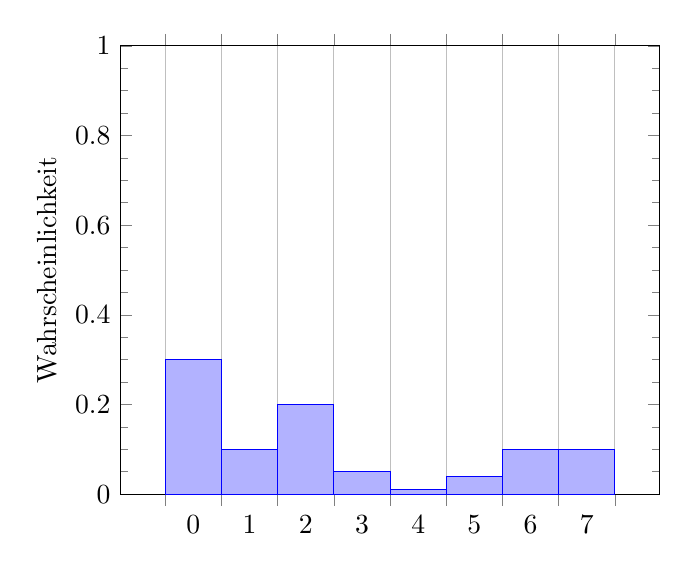
\begin{tikzpicture}
    \begin{axis}[
      ybar interval, ymax=1,ymin=0, minor y tick num = 3,
      ylabel=Wahrscheinlichkeit,]
    \addplot coordinates {(0,0.3) (1, 0.1) (2, 0.2) (3, 0.05) (4, 0.01) (5, 0.04) (6, 0.1) (7, 0.1) (8,0)};
    \end{axis}
  \end{tikzpicture}
\end{center}

\begin{Bemerkung}
  Dieses Balkendiagramm wird als Histogramm bezeichnet und ist in vielen Fällen eine gute Darstellungsmöglichkeit.
\end{Bemerkung}

\begin{GTR-Tipp}
  \begin{enumerate}
    \item Mit \texttt{seq()} (in \texttt{LIST > OPS}) wird die Liste mit allen X-Werten generiert:
    
    \texttt{seq(X,X,0,<Anzahl an Versuchen>,1)}$\rightarrow$\texttt{<Variable>}.

    ($\rightarrow$ wird durch die Taste \texttt{STO>} aufgerufen)
    \item Mit \texttt{<gewünschte Verteilung>()} (in \texttt{DISTR > DISTR}) wird die Liste mit allen Y-Werten generiert:
    
    \texttt{<Verteilung>(<Anzahl an Versuchen>,<Erfolgswahrscheinlichkeit>)}$\rightarrow$\texttt{<Variable>}.
    \item Im Menü \texttt{STAT PLOT > Plot 1} kann der gewünschte Anzeigemodus gewählt werden, für die \texttt{Xlist} wird die erste Liste gewählt, für \texttt{Freq} die zweite. Beim Anzeige achte man auf die richtigen Maßstäbe: Die Anzahl an Versuchen für \texttt{Xmax}, 1 für \texttt{Ymax}.
  \end{enumerate}

  \begin{Bemerkung}
    Der GTR ist ab einer Anzahl von über 48 überfordert, dann können die Balken wegen der niedrigen Auflösung nicht alle angezeigt werden. In einem solchen Fall kann nur ein Ausschnitt des Histogramms angezeigt werden, sonst erscheint eine Fehlermeldung.
  \end{Bemerkung}

  \begin{Bemerkung}
    Alternativ kann eine Funktion definiert werden über
    
    \texttt{<Verteilung>(<Anzahl an Versuchen>,<Erfolgswahrscheinlichkeit>,round(X,0))} und anschließend angezeigt werden.

    Dies funktionniert nur für ganze $x$, weshalb $X$ durch \texttt{round(X,0)} (zu finden in... (KP, catalog durchsuchen)) auf den nächsten ganzen Wert gerundet wird.
  \end{Bemerkung}
\end{GTR-Tipp}

\begin{Definition}[Erwartungswert]
  Es sei eine Zuffalsvariable $X$ mit Werten $x_1,x_2,...,x_n$ und die zugehörige Wahrscheinlichkeitsverteilung $P(X)$. Als Erwartungswert $\mu$ wird das arithmetische Mittel der Werte von $P(X)$ bezeichnet:
  $$E(X)=\mu=\sum_{i=1}^{n}x_i P(X=x_i)$$
\end{Definition}

\begin{Definition}[Median einer Wahrscheinlichkeitsverteilung]
  Als Median einer Wahrscheinlichkeitsverteilung bezeichnenn wir den den Wert $X_n$, ab dem die kumulierte Wahrscheinlichkeit von $P(X=x_i)$ den Wert von $50\%$ überschreitet.
\end{Definition}

\begin{Bemerkung}
  Anschaulich bezeichnet der Erwartungswert den durchschnittlichen Wert, den eine Zufallsgröße annimt, wenn ein Zufallsexperiment unendlich oft durchgeführt wird.
\end{Bemerkung}

\subsection{Binomialverteilung}
\begin{Theorem}
  Für eine Bernoulli-Kette der Länge $l \in \N$ und der Trefferwahrscheinlichkeit $P$ (Wahrscheinlichkeit für einen Pfad) gilt:
  $$P(X=k) = {l \choose k} p^k (1-p) ^{l-k}$$
  mit $k$ der gerwünschten Anzahl an Erfolgen.

  Außerdem gilt:
  $$P(X\leq k) = \sum_{i=0}^{k}{l \choose i} p^i (1-p) ^{l-i}$$
\end{Theorem}

\begin{Bemerkung}
  \begin{Definition}
    $X$ heißt in diesem Fall \textbf{binomialverteilte Zufallsvariable}. Die entsprechende Wahrscheinlichkeitsverteilung heißt Binomialverteilung. Es gilt $P(X=k) =  B_{l,p}(k)$.

    Die kumulierte Binomialverteilung wird durch ist gegeben durch: $P(X \leq k) = F_{l,p}(k)$.

    $l$ ist die Länge der Bernoulli-Kette, $p$ die Erfolgswahrscheinlichkeit und $k$ ist die gewünschte Anzahl an Erfolgen.

  \end{Definition}
\end{Bemerkung}

\begin{GTR-Tipp}
  Beide Berechnungen werden durch einen GTR-Befehl automatisiert:

  \begin{itemize}
    \item $\displaystyle{{l \choose k}} p^k (1-p) ^{l-k}$ wird duch den Befehl \texttt{binomPDF(l,p,k)} berechnet.
    \item $\displaystyle{\sum_{i=0}^{k}{l \choose i}} p^i (1-p) ^{l-i}$ wird duch den Befehl \texttt{binomCDF(l,p,k)} berechnet.
  \end{itemize}

  Beide Befehle befinden sich im \texttt{DISTR}-Menü (\texttt{2ND}+\texttt{VARS})
\end{GTR-Tipp}

\underline{Darstellung:}

\begin{minipage}{0.5\textwidth}
  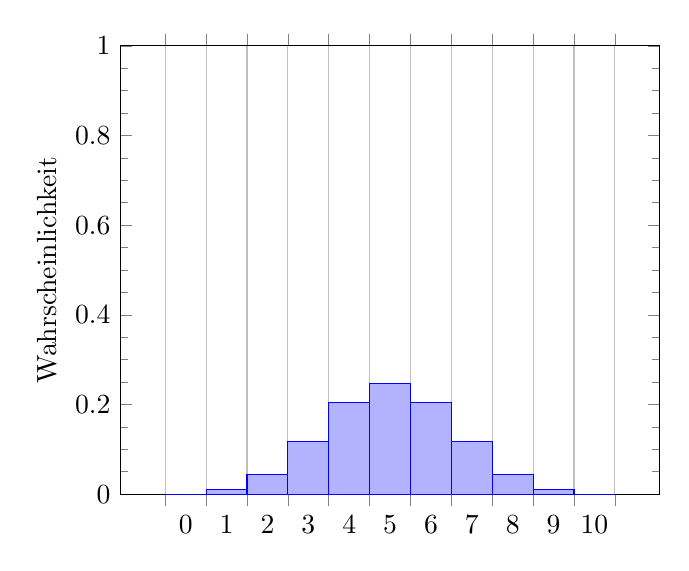
\begin{tikzpicture}
    \begin{axis}[
      ybar interval, ymax=1,ymin=0, minor y tick num = 3,
      ylabel=Wahrscheinlichkeit,]
    \addplot coordinates {(0,0) (1, 0.009765) (2, 0.04396) (3, 0.1172) (4, 0.205) (5, 0.2461) (6, 0.205) (7, 0.1172) (8, 0.04396) (9, 0.009765) (10,0) (11,0)};
    \end{axis}
  \end{tikzpicture}
\end{minipage}
\begin{minipage}{0.5\textwidth}
  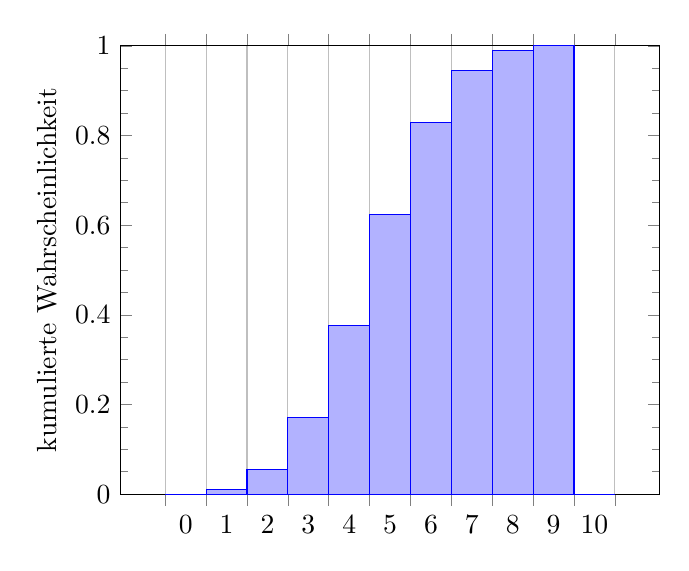
\begin{tikzpicture}
    \begin{axis}[
      ybar interval, ymax=1,ymin=0, minor y tick num = 3,
      ylabel=kumulierte Wahrscheinlichkeit,]
    \addplot coordinates {(0,0) (1, 0.0107) (2, 0.0547) (3, 0.1719) (4, 0.3770) (5, 0.623) (6, 0.8281) (7, 0.9453) (8, 0.9893) (9, 1) (10,0) (11,0)};
    \end{axis}
  \end{tikzpicture}
\end{minipage}
\subsubsection{Erwartungswert}
\begin{Theorem}[Erwartungswert einer Binomialverteilung]
  Für eine binomialverteilte Zufallsvariable $X$ gilt:
  $$E(x)=n\cdot p$$
  mit $n$ der Anzahl an Versuchen, und $p$ der Erfolgswahrscheinlichkeit eines Versuchs.
\end{Theorem}
\begin{Beweis}
  \begin{center}
    \begin{align*}
      E(x)  &= \sum_{k=0}^{n} x_k \cdot P(X=x_k)\\
            &= \sum_{k=0}^{n} k  {n \choose k} p^k (1-p)^{n-k}\\
            &= \sum_{k=0}^{n} \cdot k \dfrac{n!}{(n-k)!k!} \cdot p^k (1-p)^{n-k}\\
            &= n\cdot p\cdot \sum_{k=0}^{n} k \dfrac{(n-1)!}{(n-k-1)!k!}  p^{k-1} (1-p)^{n-k}\\
            &= n\cdot p\cdot \sum_{k=0}^{n} k  {n-1 \choose k-1} p^k (1-p)^{n-k}\\
            &= n\cdot p\cdot \sum_{k=1}^{n} k  {n-1 \choose k-1} p^k (1-p)^{n-k}\\
            &= n\cdot p \cdot 1\\
            &= n\cdot p
    \end{align*}
  \end{center}
  \begin{Bemerkung}
    Der Startindex der Summe kann verändert werden, da die kumulierte Wahrscheinlichkeit sich nicht verändert. Für $k=0$ ist ${n-1\choose k-1}=0$.
  \end{Bemerkung}
\end{Beweis}


\section{Kontinuierliche Wahrscheinlichkeiten}
Manche Ereignisse lassen sich nicht als ganze Zahl modellieren oder können nicht einzeln abgezählt werden, weshalb man ihre Wahrscheinlichkeitsverteilung nur durch kontinuierliche Funktionen darstellen kann. Man kann dies als Erweiterung der diskreten Wahrscheinlichkeit auf die reellen Zahlen sehen, analog zum Übergang von den Folgen zu den Funktionen.
\begin{Definition}[Dichtefunktion]
  Eine auf $I = [a;b]$ stetige Funktion $f$ heißt Dichtefunktion einer Wahrscheinlichkeit, wenn gilt:
  $$\int_{a}^{b} f(x)dx =1$$
\end{Definition}
\begin{Definition}
  Die Wahrscheinlichkeitsverteilung $P$, die jedem Intervall $[c;d] \subset I$ den Wert $P([c;d]) = \displaystyle \int_c^d f(x)dx$ zuordnet, heißt Wahrscheinlichkeitsverteilung über $I$.
\end{Definition}
\begin{Bemerkung}
  Durch die Definition des Integrals lassen sich folgende Eigenschaften direkt ableiten:
  \begin{itemize}
    \item $P(I)=1$
    \item $[c;d] \subset I \Rightarrow P([c;d])\in [0;1]$
    \item mit $I = [a;b]$ gilt: $P([a;c]) = 1- P([c;b])$
    \item Die Wahrscheinlichkeit eines ``Singleton'', einer ein-elementigen Menge, also eines einzelnen Ergebnisses ist:
    $P({c})=P([c;c])=\displaystyle\int_c^c f(x)dx =0$.
    \item Das bedeutet, dass $P(A \cap B)$ null sein kann, ohnen dass $A$ und $B$ disjunkt sind. (Zum Beispiel, wenn der Schnitt genau ein Element enthält.)
    \item Es folgt außerdem, dass $P([c;d])=P(]c;d])=P([c;d[)=P(]c;d[)=\displaystyle\int_c^d f(t)dt$
  \end{itemize}
\end{Bemerkung}
\begin{Definition}[Stetige Zufallsvariable]
  Sei $P$ eine Wahrscheinlichkeitsverteilung über $I$ mit Dichtefunktion $f$.

  \begin{itemize}
    \item Eine Zufallsvariable $X$ mit Werten Auswahl $I$ folgt der Wahrscheinlichkeitsverteilung $P$, wenn gilt: $$P(c\leq X \leq d)=\displaystyle \int_c^d f(t)dt$$
    \item Die Verteilungsfunktion $F$ ist definiert durch $F(X)=P(X \leq x)=P(a \leq X \leq x)=\int_a^x f(t)dt$
  \end{itemize}
\end{Definition}

\begin{Bemerkung}
  $F$ besitzt per Definition folgende Eigenschaften:
  \begin{itemize}
    \item $F$ ist differenzierbar und $F'=f$
    \item $F$ ist monoton steigend auf $I$
    \item Für $h>0$ und $x+h\in I$ gilt: $P(x \leq X \leq x+h) = F(x+h)-F(x)$.
    
    (Gleichbedeutend mit der Aussage $P(c\leq X\leq d)=F(d)-F(c)$)
  \end{itemize}
\end{Bemerkung}

\begin{Definition}[Erwartungswert]
  Sei $X$ eine Zufallsvariable mit Werten aus $I= [a;b]$. Der Erwartungswert ist gegeben durch:
  $$E(X)=\mu=\int_a^b t\cdot f(t)dt$$
\end{Definition}

\begin{Definition}[Varianz]
  Sei $X$ eine Zufallsvariable mit Werten aus $I= [a;b]$. Die Varianz ist gegeben durch:
  $$\sigma^2=\int_a^b (t-\mu)^2 \cdot f(t)dt$$
\end{Definition}


\subsection{Exponentialverteilung: $X \sim \mathcal{E}(\lambda)$}

\begin{Definition}
  Eine stetige Zufallsvariable $X$ hat eine Exponentialverteilung wenn $X$ die folgende Wahrscheinlichkeitsdichte hat:
  $$f_\lambda (x) = \lambda e^{-\lambda x}$$
  $f_\lambda(x)$ heißt Dichtefunktion der Exponentialverteilung.
\end{Definition}

\begin{Bemerkung}
  Diese Funktion erfüllt die Bedingungen der Wahrscheinlichkeitsverteilung, denn sie ist auf $\R_{+}$ definiert und stetig. Außerdem gilt: $\displaystyle \int_0^\infty f_\lambda dt = 1$.
\end{Bemerkung}

\begin{Definition}
  Die Verteilungsfunktion der Exponentialverteilung ist gegeben durch:
  $$P(X \leq x) = F_\lambda(x) = \int_{0}^{x} f_\lambda(t) dt = 1 - e^{-\lambda x}$$
\end{Definition}

\begin{Bemerkung}
  Solche Funktionen werden verwendet, um Halbwärtszeiten oder Lebensdauern zu modellieren.
\end{Bemerkung}

\begin{Theorem}[Gedächtnislosigkeit]
  Für eine exponentialverteilte Zufallsvariable $X$ gilt folgende Eigenschaft:
  $$P_{(X \geq x)}(X \geq x+t) = P(X \geq t)\qquad \forall t,x \geq 0$$
\end{Theorem}

\begin{Bemerkung}
  Das bedeutet beispielsweise für die Zersetzung eines radioaktiven Atoms, dass die Wahrscheinlichkeit sich bei $x+t$ zu zersetzen unter der Voraussetzung, dass diese noch nicht bei $x$ stattgefunden hat, nicht von $x$ abhängt.\\
  Solche Lebensdauern werden als ``alterungslos'' bezeichnet.
\end{Bemerkung}

\begin{Bemerkung}
  Die Gedächtnislosigkeit ist definierte Eigenschaft der Exponentialverteilung. (Es handelt sich somit um eine notwendige und hinreichende Bedingung)
\end{Bemerkung}

\begin{Beweis}
  \begin{align*}
    P_{(X \geq x)}(X \geq x+t) &= \dfrac{P((X \geq x)\cap(X \geq x+t))}{P(X \geq x)}\\
    &= \dfrac{P(X \geq x+t)}{P(X \geq x)}\\
    &= \dfrac{1-(1-e^{-\lambda(x+t)})}{1-(1-e^{-\lambda x})}\\
    &= \dfrac{e^{-\lambda(x+t)}}{e^{-\lambda x}}\\
    &= e^{-\lambda t}\\
    &= 1-(1-e^{-\lambda(t)})\\
    &= P(X \geq t)
  \end{align*}
\end{Beweis}

\begin{Theorem}[Erwartungswert]
  Für die Exponentialverteilung gilt:
  $$ \mu = \dfrac{1}{\lambda}$$
\end{Theorem}
\begin{Beweis}
  \begin{align*}
    \mu &= \int_0^{\infty} t \cdot f_\lambda (t)dt\\
    &= \int_0^{\infty} t \cdot \lambda e^{-\lambda t} dt\\
    &= \left[-t \cdot e^{-\lambda t}\right]_0^\infty - \int_0^{\infty} -1 \cdot e^{-\lambda t} dt\\
    &= \left[-t \cdot \lambda e^{-\lambda t}\right]_0^\infty - \left[\dfrac{1}{\lambda} e^{-\lambda t}\right]_0^\infty\\
    &= 0-0-\left(0-\dfrac{1}{\lambda}\right)\\
    &= \dfrac{1}{\lambda}
  \end{align*}
\end{Beweis}

\begin{Theorem}[Varianz]
  Für die Exponentialverteilung gilt:
  $$ \sigma^2 = \dfrac{1}{\lambda^2}$$
\end{Theorem}

\begin{Beweis}
  \begin{align*}
    \sigma^2 
    & = \int_0^{\infty} (t-\mu)^2 \cdot f_\lambda (t)dt \\
    & = \int_0^{\infty} (t-\mu)^2 \cdot \lambda e^{-\lambda t} dt \\
    & = \int_0^{\infty} t^2 \cdot \lambda e^{-\lambda t} dt - \int_0^{\infty} 2\mu t \cdot \lambda e^{-\lambda t} dt + \int_0^{\infty} \mu^2 \cdot \lambda e^{-\lambda t} dt \\
    & = \left[ -t^2 \cdot e^{-\lambda t} \right]_0^\infty - \int_0^{\infty} -2t \cdot e^{-\lambda t} dt - \left(\left[-2\mu t \cdot e^{-\lambda t}\right]_0^\infty - \int_0^{\infty} -2\mu \cdot e^{-\lambda t} dt \right) + \left[-\mu^2 \cdot e^{-\lambda t}\right]_0^\infty \\
    & = \left[-t^2 \cdot e^{-\lambda t}\right]_0^\infty - \left(\left[ \dfrac{2t}{\lambda} e^{-\lambda t}\right]_0^\infty - \int_0^{\infty} \dfrac{1}{\lambda} \cdot e^{-\lambda t} dt\right) - \left(\left[-2\mu t \cdot e^{-\lambda t}\right]_0^\infty - \left[\dfrac{2\mu}{\lambda} \cdot e^{-\lambda t}\right]_0^\infty \right) \\
    & \quad + \left[-\mu^2 \cdot e^{-\lambda t}\right]_0^\infty \\
    & = \left[-t^2 \cdot e^{-\lambda t}\right]_0^\infty - \left[\dfrac{2t}{\lambda} e^{-\lambda t}\right]_0^\infty + \left[-\dfrac{2}{\lambda^2} e^{-\lambda t}\right]_0^\infty - \left[-2\mu t \cdot e^{-\lambda t}\right]_0^\infty + \left[\dfrac{2\mu}{\lambda} \cdot e^{-\lambda t}\right]_0^\infty + \left[-\mu^2 \cdot e^{-\lambda t}\right]_0^\infty \\
    & = 0 - 0 -(0 - 0) + 0 + \dfrac{2}{\lambda^2} - (0-0) + 0 - \dfrac{2\mu}{\lambda} + 0 + \mu^2 \qquad\qquad\qquad \\
    & \quad \mu = \dfrac{1}{\lambda} \\
    & = \dfrac{2}{\lambda^2} - \dfrac{2}{\lambda^2} + \dfrac{1}{\lambda^2} \\
    & = \dfrac{1}{\lambda^2}
  \end{align*}
\end{Beweis}

\begin{Bemerkung}
  $\Rightarrow \sigma = \sqrt{\dfrac{1}{\lambda^2}} = \dfrac{1}{\lambda} = \mu$
\end{Bemerkung}


\subsection{Normalverteilung: $X \sim \mathcal{N}(\mu,\sigma^2)$}

\begin{Definition}
Eine stetige Zufallsvariable $X$ hat eine (Gauß- oder) Normalverteilung mit Erwartungswert $\mu$ und Varianz $\sigma ^{2}$ wenn $X$ die folgende Wahrscheinlichkeitsdichte hat:
$$\varphi_{\mu,\sigma^2} (x) = f(x) = \dfrac {1}{\sqrt {2\pi \sigma^2}} \cdot e^{- \dfrac{1}{2} \left( \dfrac{x-\mu}{\sigma} \right) ^2}$$
$\varphi(x)$ ist die Dichtefunktion der Normalverteilung.
\end{Definition}

\begin{Definition}
  Die Verteilungsfunktion der Normalverteilung ist gegeben durch:
  $$P(X\leq x) = \Phi_{\mu,\sigma^2}(x) = \int_{-\infty}^{x} \varphi_{\mu,\sigma^2}(t) dt$$
  Durch Substitution erhält man:
  $$\Phi_{\mu,\sigma^2}(x) = \dfrac{1}{\sqrt{2\pi}}\int_{-\infty}^{x} e^{-\frac{1}{2}t^2} dt$$
\end{Definition}

\begin{Bemerkung}
  Diese Definition ist somit analog zur Definition der Verteilungsfunktion der Binomialverteilung (Integral als Summe der Flächen).\\
  Außerdem bedeutet das, dass $\Phi(x)  \xrightarrow{\scriptscriptstyle x\rightarrow \infty} 1$.
\end{Bemerkung}

\begin{GTR-Tipp}
  Zur Berechnung geht man, wie üblich, ins Menü \texttt{DISTR} und wählt für $\varphi$  \texttt{normalpdf}, und für $\Phi$  \texttt{normalcdf} aus.
\end{GTR-Tipp}

\begin{Theorem}
  Für eine normalverteilte Zufallsvariable $X$ mit den Parametern $n,p$ und der Standardabweichung $\sigma = \sqrt{\text{Var}(X)} = \sqrt{\sigma^2}$ erhält man folgende Näherungen:
  \begin{itemize}
    \item $P(\mu - \sigma \leq X \leq \mu + \sigma) \approx 68,3\%$
    \item $P(\mu - 2\sigma \leq X \leq \mu + 2\sigma) \approx 95,4\%$
    \item $P(\mu - 3\sigma \leq X \leq \mu + 3\sigma) \approx 99,7\%$
  \end{itemize}
\end{Theorem}

\begin{Beweis}
  Die Wahrscheinlichkeit für ein bestimmtes Streuintervall $I=[\mu - z\sigma;\mu + z\sigma]$ kann berechnet werden als:
  \begin{align*}
    P(I) &= 2 \Phi(z)-1 \\
    &= 2 \dfrac{1}{\sqrt{2\pi}}\int_{-\infty}^{x} e^{-\frac{1}{2}t^2} dt -1
  \end{align*}
\end{Beweis}

\begin{Bemerkung}
  Andersherum kann die Größe von $I$ berechnet werden über:
  $$ z= \Phi^{-1} \left(\dfrac{P+1}{2}\right)$$
\end{Bemerkung}

\begin{GTR-Tipp}
  Diese Berechnung kann auch vom GTR getätigt werden: Im Menü \texttt{DISTR} wählt man \texttt{invNorm()} aus, und gibt in der Eingabe die Fläche (also die Wahrscheinlichkeit), $\mu$ und $\sigma$ an. Man erhält somit die Breite des Intervalls, und kann dies wieder in Abhängigkeit von $\sigma$ angeben.
\end{GTR-Tipp}



\subsubsection{Rückführung: Binomialverteilung}

Warum interessiert uns das? Weil die Binomialverteilung diese symmetrische Kurve für $n\rightarrow\infty$ Versuche annähert. Noch nicht überzeugt? Über die Varianz können wir interessante Aussagen über die Verteilung der Wahrscheinlichkeiten machen.

\begin{Theorem}[Laplace-Bedingung]
  Für eine Binomialverteilung mit $\sigma = \sqrt{np(1-p)}$ und $\mu = np$ gilt:\\
  Wenn $\sigma>3$, dann kann diese Binomialverteilung durch die Normalverteilung angenähert werden.
  $$B_{l,p}(k) = P(X=k) = {l \choose k} p^k (1-p) ^{l-k} \approx \varphi_{\mu,\sigma^2}(k) = \dfrac {1}{\sqrt {2\pi \sigma^2}} \cdot e^{- \dfrac{1}{2} \left(\dfrac{k-\mu}{\sigma}\right)^2};k\in \Z$$
  Daraus folgt, dass die Verteilungsfunktion ebenfalls angenähert werden kann:
  $$P(a \leq X \leq b) \approx \int_{a-0,5}^{b+a,5}\varphi_{\mu,\sigma^2}(x)dx = \Phi_{\mu,\sigma^2}(b+0,5)-\Phi_{\mu,\sigma^2}(a-0,5)$$
\end{Theorem}
\begin{Beweis}
  Die Abweichung wird so gering, dass sie vernachlässigbar wird.
\end{Beweis}
\begin{Theorem}
  Für eine binomialverteilte Zufallsvariable $X$ mit den Parametern $n,p$ und der Varianz $\sigma = \sqrt{np(1-p)}$ erhält man folgende Näherungen:
  \begin{itemize}
    \item $P(\mu - \sigma \leq X \leq \mu + \sigma) \approx 68,3\%$
    \item $P(\mu - 2\sigma \leq X \leq \mu + 2\sigma) \approx 95,4\%$
    \item $P(\mu - 3\sigma \leq X \leq \mu + 3\sigma) \approx 99,7\%$
  \end{itemize}
\end{Theorem}

TODO:
\section{Hypothesen}
\subsection{Signifikanztests}
\subsubsection{Einseitiger Test}
\subsubsection{Zweiseitiger Test}
\subsection{Hypothesentests}
\subsubsection{Fehler 1. Art}
\subsubsection{Fehler 2. Art}

\end{document}
